\chapter{Interpolación}
\section{Interpolación Polinómica}
En esta sección, resolvemos el siguiente problema: Se nos da una tabla de $n + 1$ puntos de datos $(x_i, y_i)$ y buscamos un polinomio $p$ de menor grado posible tal que $p(x_i) = y_i \quad (0 \leq i \leq n)$. Dicho polinomio se dice que interpola los datos. Aquí está el teorema que rige este problema.

\begin{theorem}
Si $x_0, x_1,..., x_n$ son números reales distintos, entonces para valores arbitrarios $y_0, y_1,..., y_n$ hay un único polinomio $p_n$ de grado como mucho $n$ tal que
\[ p_n(x_i) = y_i \quad (0 \leq i \leq n) \]
\end{theorem}

\begin{proof}
Demostraremos primero la unicidad. Supongamos que existieran dos tales polinomios, \( p_n \) y \( q_n \). Entonces, el polinomio \( p_n - q_n \) tendría la propiedad de que \( (p_n - q_n)(x_i) = 0 \) para \( 0 \leq i \leq n \). Dado que el grado de \( p_n - q_n \) puede ser como máximo \( n \), este polinomio puede tener como máximo \( n \) ceros si no es el polinomio nulo. Como los \( x_i \) son distintos, \( p_n - q_n \) tiene \( n + 1 \) ceros; por lo tanto, debe ser cero. Así, \( p_n \equiv q_n \).    

Para la parte de existencia del teorema, procedemos inductivamente. Para \( n = 0 \), la existencia es obvia ya que se puede elegir una función constante \( p_0 \) (polinomio de grado \( \leq 0 \)) tal que \( p_0(x_0) = y_0 \). Ahora supongamos que hemos obtenido un polinomio \( p_{k-1} \) de grado \( \leq k - 1 \) con \( p_{k-1}(x_i) = y_i \) para \( 0 \leq i \leq k - 1 \). Intentamos construir \( p_k \) de la forma
\begin{equation}
    \label{eq: Kincaid 1}
    p_k (x) = p_{k - 1} (x) + c (x - x_0) (x - x_1) ... (x-x_{k - 1})
\end{equation}

Observa que esto es, sin lugar a dudas, un polinomio de grado como máximo \( k \). Además, \( p_k \) interpola los datos que interpola \( p_{k-1} \), porque
\[ p_k(x_i) = p_{k - 1} (x_i) = y_i \quad (0 \leq i \leq k -1)\]
Ahora determinamos el coeficiente desconocido \( c \) a partir de la condición \( p_k(x_k) = y_k \). Esto conduce a la ecuación
\begin{equation}
    \label{eq: Kincaid 2}
    p_{k - 1}(x_k) + c(x_k - x_0) (x_k - x_1)...(x_k - x_{k - 1} = y_k)
\end{equation}

La ecuación \ref{eq: Kincaid 2} ciertamente puede resolverse para \( c \) porque los factores que multiplican a \( c \) no son cero.

\end{proof}

\subsection{Forma de Newton del Polinomio de Interpolación}

Antes de intentar escribir un algoritmo que lleve a cabo el proceso recursivo en esta demostración, necesitamos hacer algunas observaciones. En primer lugar, los polinomios \( p_0, p_1, \ldots, p_n \) construidos en la demostración tienen la propiedad de que cada \( p_k \) se obtiene simplemente añadiendo un término a \( p_{k-1} \). Por lo tanto, al final del proceso, \( p_n \) será una suma de términos y cada \( p_0, p_1, \ldots, p_{n-1} \) será claramente visible en la expresión para \( p_n \). Cada \( p_k \) tiene la forma
\begin{equation}
    \label{eq: Kincaid 3}
    \resizebox{0.5 \textwidth}{!}{$p_k(x) = c_0 + c_1 (x - x_0) + c_2 (x - x_0) (x - x_1) + ... + c_k (x - x_0) ...(x - x_{k - 1})$}
\end{equation}

Su forma compacta es
\begin{equation}
    \label{eq: Kincaid 4}
    p_k (x) = \sum_{i = 0}^{k} c_i \prod_{j = 0}^{i - 1} (x - x_j)
\end{equation}

Estos polinomios se denominan polinomios de interpolación en la forma de Newton.

\subsection{Forma de Lagrange del Polinomio de Interpolación}
Ahora presentamos una forma alternativa para el polinomio de interpolación \( p \) asociado con una tabla de puntos de datos \((x_i, y_i)\) para \( 0 \leq i \leq n \). Es importante entender que existe un único polinomio de interpolación de grado \(\leq n\) asociado con los datos. Sin embargo, ciertamente existe la posibilidad de expresar este polinomio en diferentes formas y de llegar a él mediante distintos algoritmos.

El método alternativo expresará \( p \) en la forma
\begin{equation}
    \label{eq: Kincaid 9}
    p(x) = y_0 l_o(x) + y_1 l_1(x) +...+ y_n l_n(x) = \sum_{k = 0}^{n} y_k l_k(x)
\end{equation}
Aquí \( l_0, l_1, \ldots, l_n \) son polinomios que dependen de los nodos \( x_0, x_1, \ldots, x_n \) pero no de las ordenadas \( y_0, y_1, \ldots, y_n \).  
Dado que las ordenadas podrían ser todas 0 excepto por un 1 ocupando la posición \( i \)-ésima, vemos que
\[ \delta_{ij} = p_n (x_j) = \sum_{k = 0}^{n} y_k l_k(x_j) = \sum_{k = 0}^{n} \delta_{ki} l_k(x_j) = l_i(x_j) \]

La fórmula general de \( l_i \) es
\begin{equation}
    \label{eq: Kincaid 10}
    l_i(x) = \prod_{j = 0 \atop j \neq 0}^{n} \frac{x - x_j}{x_0 - x_j} \quad (0 \leq i \leq n)
\end{equation}
Para el conjunto de nodos \( x_0, x_1, \ldots, x_n \), estos polinomios son conocidos como las funciones cardinales. Con los polinomios cardinales en mano, la Ecuación \ref{eq: Kincaid 9} proporciona la forma de Lagrange de los polinomios interpolantes.

Existen aún otros algoritmos para la interpolación polinómica, y estos tienen diversas ventajas y desventajas. Dado que existe un único polinomio de grado \(\leq n\) que toma valores prescritos en \(n + 1\) puntos dados (y distintos), estos algoritmos producen el mismo polinomio en diferentes formas. Por ejemplo, podemos requerir que nuestro polinomio se exprese en potencias de \(x\):
\begin{equation}
    \label{eq: Kincaid 11}
    p(x) = a_0 + a_1 x + a_2 x^2 + ... + a_n x^n
\end{equation}

Las condiciones de interpolación, \( p(x_i) = y_i \) para \( 0 \leq i \leq n \), conducen a un sistema de \( n + 1 \) ecuaciones lineales para determinar \( a_0, a_1, \dots, a_n \). Este sistema tiene la forma:
\begin{equation}
    \label{eq: Kincaid 12}
    \begin{bmatrix}
        1       &       x_0     &       x_0^2       &       \dots       &       x_0^n       \\
        1       &       x_1     &       x_1^2       &       \dots       &       x_1^n       \\
        1       &       x_2     &       x_2^2       &       \dots       &       x_2^n       \\
        \vdots  &       \vdots  &       \vdots      &       \ddots      &       \vdots      \\
        1       &       x_n     &       x_n^2       &       \dots       &       x_n^n       \\
    \end{bmatrix}
    \begin{bmatrix}
        a_0 \\
        a_1 \\
        a_2 \\
        \vdots \\
        a_n
    \end{bmatrix} = 
    \begin{bmatrix}
        y_0 \\
        y_1 \\
        y_2 \\
        \vdots \\
        y_n 
    \end{bmatrix}
\end{equation}

La matriz de coeficientes aquí se llama matriz de Vandermonde. Es no singular porque el sistema tiene una solución única para cualquier elección de \( y_0, y_1, \dots, y_n \). El determinante de la matriz de Vandermonde, por lo tanto, es no nulo para nodos distintos \( x_0, x_1, \dots, x_n \). Sin embargo, la matriz de Vandermonde a menudo está mal condicionada, por lo que los coeficientes \( a_i \) pueden ser determinados de manera imprecisa al resolver el Sistema \ref{eq: Kincaid 12}. Además, la cantidad de trabajo necesario para obtener el polinomio en \ref{eq: Kincaid 11} es excesiva. Por lo tanto, este enfoque no se recomienda.

\subsection{El Error en la Interpolación Polinómica}
Ahora presentamos algunos teoremas que se refieren a la discrepancia entre una función y un polinomio interpolante de esta.
\begin{theorem}
\label{teo: Kincaid 2}
Sea \( f \) una función en \( C^{n + 1}[a, b] \), y sea \( p \) el polinomio de grado \(\leq n\) que interpola la función \( f \) en \( n + 1 \) puntos distintos \( x_0, x_1, \ldots, x_n \) en el intervalo \([a, b]\). Para cada \( x \) en \([a, b]\), existe un punto \( \xi_x \) en \((a, b)\) tal que
\begin{equation}
    \label{eq: Kincaid 13}
    f(x) - p(x) = \frac{1}{(n + 1)!} f^{(n + 1)} (\xi_x) \prod_{i = 0}^{n} (x - x_i)
\end{equation}
\end{theorem}

\begin{proof}
Si \( x \) es uno de los nodos de interpolación \( x_i \), la afirmación es obviamente verdadera, ya que ambos lados de la Ecuación \ref{eq: Kincaid 13} se reducen a cero. Entonces, sea \( x \) cualquier punto distinto de un nodo. Definamos
\[ w(t) = \prod_{i = 0}^{n} (t - x_i) \quad \phi \equiv f - p - \lambda w \]
donde \( \lambda \) es el número real que hace que \( \phi(x) = 0 \). Por lo tanto,
\[ \lambda = \frac{f(x) - p(x)}{w(x)} \]

Ahora $\phi \in C^{n + 1} [a, b]$ y $\phi$ se anula en los puntos $n + 2$ $x, x_0, x_1,...,x_n$. Por el Teorema de Rolle, $\phi'$ tiene al menos $n + 1$ ceros distintos en $(a, b)$. De manera similar, $\phi''$ tiene al menos $n$ ceros distintos en $(a, b)$. Si este argumento se repite, concluimos eventualmente que $\phi^{(n + 1)}$ tiene al menos un cero, digamos $\xi_x$, en $(a, b)$. Ahora
\[ \phi^{(n + 1)} = f^{(n + 1)} - p^{(n + 1)} - \lambda w^{(n + 1)} = f^{(n + 1)} - (n + 1)! \lambda\]
Entonces

\noindent \resizebox{0.5 \textwidth}{!}{$0 = \phi^{(n + 1)}(\xi_x) = f^{(n + 1)}(\xi_x) - (n + 1)! \lambda = f^{(n + 1)}(\xi_x) - (n + 1)! \frac{f(x) - p(x)}{w(x)}$}
\end{proof}

\subsection{Polinomios de Chebychev}
En el Teorema \ref{teo: Kincaid 2}, hay un término que puede optimizarse eligiendo los nodos de una manera especial. El proceso de optimización conduce naturalmente a un sistema de polinomios llamados polinomios de Chebyshev, y comenzamos con su definición y propiedades básicas.

Los polinomios de Chebyshev se definen recursivamente de la siguiente manera:
\begin{equation}
    \begin{cases}
        T_0 (x) = 1 \quad T_1(x) = x \\
        T_{n + 1}(x) = 2xT_n(x) - T_{n - 1}(x) \quad (n \geq 1)
    \end{cases}
\end{equation}

\begin{theorem}
\label{teo: Kincaid 3}
Para $x$ en el intervalo $[-1, 1]$, los polinomios de Chebyshev tienen la siguiente expresión en forma cerrada:
\[ T_n(x) = cos(n cos^{-1}x) \quad (n \geq 0)\] 
\end{theorem}

\begin{theorem}
\label{teo: Kincaid 4}
Si $p$ es un polinomio mónico de grado $n$, entonces
\[ \|p\|_\infty = \max_{-1 \leq x \leq 1} |p(x)| \geq 2^{1 - n} \]
\end{theorem}

\begin{proof}
Procedemos por contradicción. Supongamos que
\[ |p(x)| < 2^{1 - n} \quad (|x| \leq 1) \]
Sea $q = 2^{1 - n} T_n$ y $x_i = cos(i\pi / n)$. Como se señaló anteriormente, $q$ es un polinomio mónico de grado $n$. Entonces
\[ (-1)^i p(x_i) \leq |p(x_i)| < 2^{1 - n} = (-1)^i q(x_i) \]
En consecuencia
\[ (-1)^i [q(x_i) - p(x_i)] > 0 \quad (0 \leq i \leq n) \]
Esto muestra que el polinomio \( q - p \) oscila en signo \( n+1 \) veces en el intervalo \([-1, 1]\). Por lo tanto, debe tener al menos \( n \) raíces en \((-1, 1)\). Pero esto no es posible porque \( q - p \) tiene grado como máximo \( n - 1 \).
\end{proof}

\subsection{Eligiendo los Nodos}
En el Teorema \ref{teo: Kincaid 2}, supongamos que los nodos de interpolación están en el intervalo \([-1, 1]\). Si \( x \) está en este mismo intervalo, \( \xi_x \) también estará en ese intervalo. Por lo tanto, podemos deducir que
\noindent \resizebox{0.5 \textwidth}{!}{$\max_{|x| \leq 1} |f(x) - p(x)| \leq \frac{1}{(n + 1)!} \max_{|x| \leq 1} |f^{(n + 1)}(x)| \max_{|x| \leq 1} \left| \prod_{i = 0}^{n} (x - x_i) \right|$}
Por el Teorema \ref{teo: Kincaid 4}, tenemos
\[ \max_{|x| \leq 1} \left| \prod_{i = 0}^{n} (x - x_i) \right| \geq 2^{-n} \]
Este valor mínimo se alcanzará si $\prod_{i = 0}^{n} (x - x_i)$ es el múltiplo monico de
$T_{n + 1}$; que es, $2^{-n}T_{n + 1}$. Los modos serán entonces las raíces de \( T_{n+1} \). Estas son
\[ x_i = cos \left( \frac{2i + 1}{2n + 2} \pi \right) \quad (0 \leq i \leq n) \]
Estas consideraciones establecen el siguiente resultado.
\begin{theorem}
Si los nodos \( x_i \) son las raíces del polinomio de Chebyshev \( T_{n+1} \), entonces la fórmula de error en el Teorema 2 da (para \( |x| \leq 1 \)):

\[ |f(x) - p(x)| \leq \frac{1}{2^n (n+1)!} \max_{|t| \leq 1} |f^{(n + 1)}(t)| \]
    
\end{theorem}

\subsection{El Teorema de Aproximación de Weiertrass}
\begin{theorem}
    Si $f$ es continua en $[a, b]$ y si $\epsilon > 0$, existe un polinomio $p$ tal que $|f(x) - p(x)| \leq \epsilon$ en el intervalo $[a, b]$.
\end{theorem}

\section{Interpolación Unidimensional}
El alcance de esta sección es la teoría de la interpolación de funciones definidas en un intervalo $[a, b]$. Para un entero $k \geq 0$, $\mathbb{P}_k$ denota el espacio de los polinomios en una variable, con coeficientes reales y de grado a lo sumo $k$.

\subsection{La malla}
Una malla de $\Omega = [a, b]$ es una colección indexada de intervalos de medida no nula $\left\{ I_i = [x_{1, i}, x_{2, i}] \right\}_{0 \leq i \leq N}$ que forma una partición de $\Omega$, es decir,
\begin{equation}
    \label{eq: TAMU 1.1}
    \bar{\Omega} = \cup_{i = 0}^{N} I_i \quad \text{y} \quad \mathring{I_i} \cap \mathring{I_j} = \emptyset \quad \text{para} \quad i \neq j
\end{equation}

La forma más sencilla de construir una malla es tomar $N + 2$ puntos en $\Omega$ tal que
\begin{equation}
    \label{eq: TAMU 1.2}
    a = x_0 < x_1 <...<x_N < x_{N + 1} = b
\end{equation}
y definir $x_{1, i} = x_i$ y $x_{2,i} = x_{i + 1}$ para $0 \leq i \leq N$. Los puntos en el conjunto $\{ x_0, ..., x_{N + 1} \}$ se llaman los vértices de la malla. El mallado puede tener tamaño de paso variable 
\[ h_i = x_{i + 1} - x_i \quad 0 \leq i \leq N \]
y establecemos
\[ h = \max_{0 \leq i \leq N} h_i \]

En lo sucesivo, los intervalor $I_i$ también se llaman elementos (o celdas) y la malla se denota por $T_h = \{ I_i \}_{0 \leq i \leq N}$. El subíndice $h$ hace referencia al nivel de refinamiento.

\subsection{El elemento finito $\mathbb{P}_1$ de Lagrange}
Considera el espacio vectorial de funciones continuas, lineales a trozos 
\begin{equation}
    \label{eq: TAMU 1.3}
    P_h^1 = \{ v_h \in C^0(\bar{\Omega}); \forall i \in \{ 0,...,N \}, v_{h|I_i} \in \mathbb{P}_1 \}
\end{equation}
Este espacio puede ser utilizado en conjunto con los métodos de Garlekin para aproximar ecuaciones en derivadas parciales unidimensionales. Por esta razón, $P_1^h$ se llama un espacio de aproximación. Introducimos las funciones $\{ \phi_0,..., \phi_{N + 1} \}$ definidas elemento por elemento como sigue: Para $i \in \{ 0,..., N + 1 \}$
\begin{equation}
    \label{eq: TAMU 1.4}
    \phi_i(x) = \begin{cases}
        \frac{1}{h_{i - 1}}(x - x_{i-1}) \quad \text{si } x \in I_{i - 1} \\
        \frac{1}{h_i}(x_{i + 1} - x) \quad \text{si } x \in I_i \\
        0 \quad \text{en otro caso}
    \end{cases}
\end{equation}
con modificaciones obvias si $i = 0$ o $i = N + 1$. Claramente, $\phi_i \in P_i^h$. Estas funciones son comúnmente llamadas ``funciones de sombrero'' debido a la forma de su gráfico; véase la figura \ref{fig: Funciones de Sombrero Unidimensionales}.

\begin{figure}[h]
    \centering
    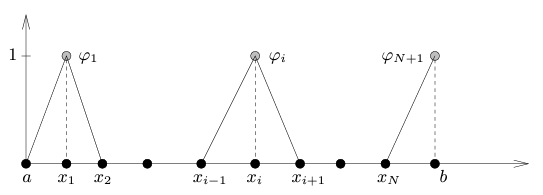
\includegraphics[width = 0.5 \textwidth]{Imagenes/4 - Funciones de Sombrero Unidimensionales.png}
    \caption{Funciones de Sombrero Unidimensionales}
    \label{fig: Funciones de Sombrero Unidimensionales}
\end{figure}

\subsection{El elemento finito $\mathbb{P}_k$ de Lagrange}
La técnica de interpolación presentada en la sección 2.2 se generaliza a polinomios de mayor grado. Consideremos la malla $\tau_h = \{I_i\}_{0 \leq i \leq N}$ introducida en la sección 2.1. Sea 
\begin{equation}
    \label{eq: TAMU 1.14}
    P_h^k = \{ v_h \in C^0 (\bar{\Omega}); \forall i \in \{ 0,..., N \}, v_{h|I_i} \in \mathbb{P}_k \}
\end{equation}

Para investigar un operador de interpolación con codominio en $P_h^k$, es conveniente considerar los polinomios de Lagrange. Recuerda lo siguiente:

\begin{definition}
    \textbf{Polinomios de Lagrange} Sea $k \geq 1$ y $\{ s_0, ..., s_k \}$ un conjunto de $k + 1$ números distintos. Los polinomios de Lagrange $\{ \mathcal{L}_0^k, ..., \mathcal{L}_k^k \}$ asociados con los nodos $\{ s_0, ..., s_k \}$ se definen como 
    \begin{equation}
        \label{eq: TAMU 1.15}
        \mathcal{L}_m^k(t) = \frac{\prod_{l \neq m} (t - s_l)}{\prod_{l \neq m}(s_m - s_l)}, \quad 0 \leq m \leq k
    \end{equation}
\end{definition}

Los polinomios de Lagrange cumplen la propiedad importante
\[ \mathcal{L}_m^k (s_l) = \delta_{ml}, \quad 0 \leq m, l \leq k \]

La Figura \ref{fig: Familias de Polinomios de Lagrange} presenta familias de polinomios de Lagrange con nodos equidistribuidos en el intervalo de referencia $[0, 1]$ para $k = 1, 2$ y $3$.

\begin{figure}[h]
    \centering
    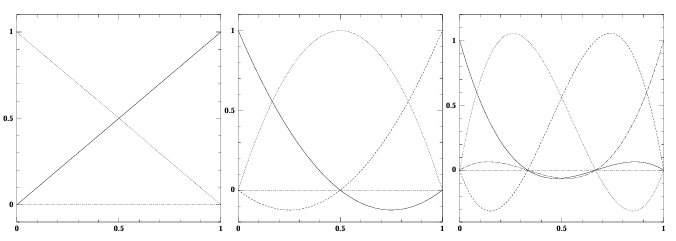
\includegraphics[width = 0.5 \textwidth]{Imagenes/4 - Familias de Polinomios de Lagrange.png}
    \caption{Familias de polinomios de Lagrange con nodos equidistribuidos en el intervalo de referencia $[0, 1]$ y de grado $k = 1$ (izquierda), $k = 2$ (centro) y $k = 3$ (derecha).}
    \label{fig: Familias de Polinomios de Lagrange}
\end{figure}

Para $i \in \{ 0,..., N \}$, introducimos los nodos $\xi_{i, m} = x_i + m \frac{h_i}{k}$, $0 \leq m \leq k$, en el intervalo de la malla $I_i$. Sea $\{ \mathcal{L}_{i, 0}^k,..., \mathcal{L}_{i, k}^k \}$ el conjunto de polinomios de Lagrange asociados con estos nodos. Para $j \in \{ 0,..., k(N + 1) \}$ con $j = ki + m$ y $0 \leq m \leq k - 1$, definimos la función $\phi_j$ elemento a elemento de la siguiente manera: Para $º \leq m \leq k - 1$
\[ \phi_{ki + m}(x) = \begin{cases}
    \mathcal{L}_{i, m}^k (x) \quad \text{si } x \in I_i \\
    0   \quad \text{ en caso contrario}
\end{cases} \]
y para $m = 0$,
\[ \phi_{ki}(x) = \begin{cases}
    \mathcal{L}_{i, 0}^k(x) \quad \text{ si } x \in I_i \\
    \mathcal{L}_{i - 1, k}^k(x) \quad \text{ si } x \in I_{i - 1} \\
    0 \quad \text{ en caso contrario }
\end{cases} \]
con modificaciones evidentes si $i = 0$ o $i = N + 1$. Las funciones $\phi_j$ se ilustran en la Figura \ref{fig: phij para k2} para $k = 2$. Obsérvese la diferencia entre el soporte de las funciones asociadas a los vértices de la malla (dos intervalos adyacentes) y el de las funciones asociadas a los puntos medios de las celdas (un intervalo).
\begin{figure}[h]
    \centering
    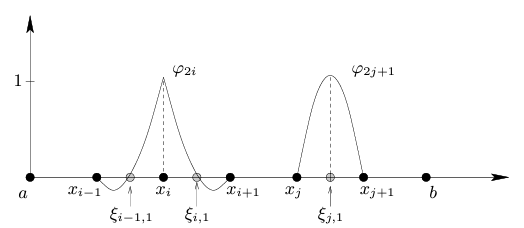
\includegraphics[width = 0.5 \textwidth]{Imagenes/4 - Funciones de forma globales en el espacio de aproximacion Ph2.png}
    \caption{Funciones de forma globales en el espacio de aproximación $P_h^2$.}
    \label{fig: phij para k2}
\end{figure}

\section*{Ejercicios}
\noindent (1) Sea $f(x) = (3 + x) cos^2(\pi x /4)$, $x \in [0, 3]$. Utilizar el polinomio interpolador de Lagrange cuadrático con nodos $x_1 = 0, x_2 = 1, x_3 = 3$ para aproximar $f(2)$, $f(12/5)$, $f(7/2)$ y $f(4)$.

\noindent (2) Para las siguientes funciones $f(x)$, escribir el término del error $E_2(x)$ del polinomio interpolador de Lagrange cuadrático con nodos $x_0 = -1, x_1 = 1, x_2 = 3$.
\begin{itemize}
    \item $f(x) = 4 x^2 - 3x + 2$
    \item $f(x) = x^3 - 2 x^2 + 1$
\end{itemize}

\noindent (3) Aproximar el valor $0.15^{1/7}$ mediante el polinomio interpolador cuadrático de la función $f(x) = 2^x$ con los nodos $x_0 = -1, x_1 = 0, x_2 = 1$. Acotar el error cometido.

\noindent (4) ¿Cuál es el polinomio interpolaor de Lagrange de grado 21 con nodos equidistantes, de la función $f(x) = x^5 + 3 x^{12}$, $x \in [0, 20]$.

\noindent (5) Se considera la función $f(x) = \frac{1}{1 + x^2}$. Calcular y representar gráficamente el polinomio de interpolación de grado 14 con puntos de interpolación equiespaciados en el intervalo $[-5 , 5]$.

\noindent (6) Haciendo uso de la transformación lineal $F: [-1 , 1] \rightarrow [-5, 5]$, con $F(x) = 5x$, repetir el ejercicio anterior utilizando como puntos de interpolación $x_i = F(\hat{x}_i)$, donde los puntos
\[ \hat{x}_i = cos\left( \frac{2i + 1}{2n + 2} \pi \right) 0 \leq i \leq n \]

\noindent (7) Dado el intervalo $[0, 2]$, se genera un mallado $D_h$ formado por elementos de anchura $h = 0.5$, y sea $V_h$ el esapcio de elementos finitos generado con polinomios de grado 1 o 2. Se considera la función $f: [0, 2] \rightarrow \mathbb{R}$ dad por $f(x) = sin(\pi x)$ y sea $f_h \in V_h$ una aproximación de $f$ en el espacio $V_h$ verificando que $f(x_i) = f_h (x_i)$ para todo $x_i$ nodo del mallado. Se piede:
\begin{itemize}
    \item Calcular $|f(0.8) - f_h(0.8)|$
    \item Repetir el ejercicio utilizando $h = 1/2^j$, $j = 2, 3, 4$.
    \item Para qué valor de $h$ podemos afirmar que el error está por debajo de una tolerancia de $\delta = 10^{-6}$.
\end{itemize}

\noindent (8) Determinar el valor de $h$ para que la aproximación $f_h \in V_h$ de la función $f$ verifique que 
\[ \|f - f_h\|_{L^\infty ([a, b])} < \delta \]
suponiendo que el mallado asociado a $V_h$ es equiespaciado, que el grado de los polinomios para construir $V_h$ es $m = 1$ o $2$, que $\delta = 10^{-8}$ y para las siguientes funciones $f$:
\begin{itemize}
    \item $f:[0, 10] \rightarrow \mathbb{R}$, $f(x) = x sin x$
    \item $f:[-1, 1] \rightarrow \mathbb{R}$, $f(x) = sin(\pi x)$
    \item $f:[-1, 1] \rightarrow \mathbb{R}$, $f(x) = x arctg x$
    \item $f:[-5, 5] \rightarrow \mathbb{R}$, $f(x) = e^{-x^2}$
\end{itemize}